%%%%%%%%%%%%%%%%%%%%%%%%%%%%%%%%%%%%%%%%%%%%%%%%%%%%%
%												    %
%	VIAGEM PELA EUROPA  						    %
%												    %
%	Abril 2015									    %
%												    %
%	Angela Cardodo, Felipe Galvão e Bruno Madeira	%
%   											    %	
%%%%%%%%%%%%%%%%%%%%%%%%%%%%%%%%%%%%%%%%%%%%%%%%%%%%%

\documentclass[12pt,a4paper,reqno]{report}
\linespread{1.5}

\usepackage[active]{srcltx}    
\usepackage{graphicx}
\usepackage{amsthm,amsfonts,amsmath,amssymb,indentfirst,mathrsfs,amscd}
\usepackage[mathscr]{eucal}
\usepackage[active]{srcltx} %inverse search
\usepackage{tensor}
\usepackage[utf8x]{inputenc}
\usepackage[portuges]{babel}
\usepackage[T1]{fontenc}
\usepackage{enumitem}
\setlist{nolistsep}
\usepackage{comment} 
\usepackage{tikz}
\usepackage[numbers,square, comma, sort&compress]{natbib}
%\numberwithin{figure}{section}
\numberwithin{equation}{section}
\usepackage{scalefnt}
\usepackage[top=2.5cm, bottom=2.5cm, left=2.5cm, right=2.5cm]{geometry}
%\usepackage{tweaklist}
%\renewcommand{\itemhook}{\setlength{\topsep}{0pt}%
%	\setlength{\itemsep}{0pt}}
%\renewcommand{\enumhook}{\setlength{\topsep}{0pt}%
%	\setlength{\itemsep}{0pt}}
%\usepackage[colorlinks]{hyperref}
\usepackage{MnSymbol}
%\usepackage[pdfpagelabels,pagebackref,hypertexnames=true,plainpages=false,naturalnames]{hyperref}
\usepackage[naturalnames]{hyperref}
\usepackage{enumitem}
\usepackage{titling}
\newcommand{\subtitle}[1]{%
	\posttitle{%
	\par\end{center}
	\begin{center}\large#1\end{center}
	\vskip0.5em}%
}
\newcommand{\HRule}{\rule{\linewidth}{0.5mm}}
\usepackage{caption}
\usepackage{etoolbox}% http://ctan.org/pkg/etoolbox
\usepackage{complexity}

\usepackage[official]{eurosym}

\def\Cpp{C\raisebox{0.5ex}{\tiny\textbf{++}}}

\makeatletter
\def\@makechapterhead#1{%
  %%%%\vspace*{50\p@}% %%% removed!
  {\parindent \z@ \raggedright \normalfont
    \ifnum \c@secnumdepth >\m@ne
        \huge\bfseries \@chapapp\space \thechapter
        \par\nobreak
        \vskip 20\p@
    \fi
    \interlinepenalty\@M
    \Huge \bfseries #1\par\nobreak
    \vskip 40\p@
  }}
\def\@makeschapterhead#1{%
  %%%%%\vspace*{50\p@}% %%% removed!
  {\parindent \z@ \raggedright
    \normalfont
    \interlinepenalty\@M
    \Huge \bfseries  #1\par\nobreak
    \vskip 40\p@
  }}
\makeatother


\begin{document}



\begin{titlepage}
\begin{center}
 
\vspace*{3cm}

{\Large Concepção e Análise de Algoritmos}\\[2cm]

% Title
{\Huge \bfseries Troca de Letras \\[1cm]}

% Author
{\large Ângela Cardoso e Bruno Madeira}\\[2cm]


\includegraphics[width=10cm]{feup_logo.jpg}\\[2cm]


% Bottom of the page
{\large \today}

\end{center}
\end{titlepage}

\tableofcontents


%%%%%%%%%%%%%%
% INTRODUCAO %
%%%%%%%%%%%%%%
\chapter{Introdução}

No âmbito da disciplina de Concepção e Análise de Algoritmos do Mestrado Integrado em Engenharia Informática e Computação, foi-nos proposta a resolução de um problema cuja formulação é frequentemente feita através da utilização de grafos.

O tema do nosso projeto é o planeamento de uma viagem pela Europa. Mais precisamente, o cliente pretende visitar várias cidades europeias, deslocando-se de carro entre elas. Tem um tempo máximo predefinido para realizar a viagem, assim como uma classificação das cidades consoante o seu interesse, numa pontuação de 0 (pouco interessado) a 10 (muito interessado). Além disso, o cliente disponibiliza informação sobre o tempo de deslocação entre as cidades, assim como o tempo que demora a visitar cada uma delas. A solução a devolver ao cliente será uma lista ordenada de cidades a visitar, tendo em conta que começa e acaba na cidade onde reside.

Numa versão inicial do problema, o tempo para a viagem é limitado e, como tal, poderá não ser possível ir a todas as cidades, o objetivo é visitar as cidades mais interessantes. Numa outra versão, será calculado o tempo mínimo necessário para visitar todas as cidades, sendo devolvido o percurso mais eficiente.

Numa primeira parte do projeto apresentou-se uma formulação matemática do problema, incluindo as restrições assumidas. Expuseram-se ainda esboços de possíveis resoluções, exatas e aproximadas, para as duas versões do problema, assim como propostas de análise do custo computacional dos algoritmos propostos e da qualidade das aproximações.

Nesta fase final, foram concretizadas várias das resoluções discutidas, mas também outras que não tinham sido apresentadas. Analisou-se experimentalmente a complexidade temporal dos algoritmos implementados, assim como a qualidade das soluções heurísticas. Tudo isto, assim como o que tinha sido feito anteriormente, é exposto no presente documento.

%%%%%%%%%%%%%%
% RESTRIÇÕES %
%%%%%%%%%%%%%%
\chapter{Limites de Aplicabilidade}

Cada instância do nosso problema é representada por um grafo, em que os vértices correspondem às cidades a visitar e as arestas correspondem aos percursos entre as cidades. Apesar de esta representação já contemplar uma série de aspetos do problema, existem ainda várias alternativas consoante os dados fornecidos e as restrições que sejam consideradas. A menos que algo seja dito explicitamente em contrário, à partida, o ideal será não impor restrições que limitem a aplicabilidade dos algoritmos desenvolvidos. Por outro lado, existem casos em que a limitação é recompensada pela eficiência dos algoritmos possíveis.

No caso do planeamento de uma viagem, há três questões que devem ser respondidas, por forma a identificar eventuais restrições a considerar:
\begin{enumerate}
	\item Dadas duas cidades, existe sempre um caminho que as une sem passar por nenhuma outra cidade da lista? Isto é, podemos considerar um grafo completo?
	\item Dado um caminho que une as cidades A e B, existe alguma diferença entre ir de A para B ou de B para A? Isto é, teremos que considerar um grafo dirigido ou não?
	\item Podemos assumir que dadas três cidades A, B e C, o tempo de viagem de [A, C] nunca é maior que a soma dos tempos de [A, B] e [B, C]? Isto é, a desigualdade triangular é válida nos custos associados às arestas do grafo?
\end{enumerate}

Apesar de não ser dito de forma explícita, iremos assumir que o grafo é completo, porque não se trata de uma verdadeira restrição para este problema específico. De facto, se não existisse um caminho direto entre as cidades A e C e fosse sempre necessário passar por B, poderíamos considerar uma nova aresta entre A e C, cujo tempo de percurso é a soma dos tempos [A, B] e [B, C]. Na prática isto corresponderia a ir de A para C passando pela cidade B, mas sem a visitar.

Tipicamente, dentro de localidades, existem diferenças entre ir do ponto A para o ponto B ou fazer o percurso inverso. Já neste caso, à partida não seria muito restritivo assumir que não é necessário considerar arestas dirigidas, porque os tempos de deslocação serão relativamente grandes e pequenas diferenças devidas à orientação poderiam ser desprezadas. No entanto, uma vez que também é necessário considerar o tempo de visita de cada cidade a que chegamos, iremos considerar arestas dirigidas, cujo custo incluirá, além do tempo de viagem, o tempo de visita da cidade de destino. Ora, uma vez que os grafos considerados serão dirigidos, podemos perfeitamente permitir que os tempos sejam diferentes consoante se vá num sentido ou noutro. Convém no entanto notar que, ao considerar grafos completos dirigidos, teremos o dobro das arestas, em relação à versão do problema não dirigido. Este crescimento do grafo poderá ter um impacto negativo na eficiência dos algoritmos desenvolvidos.

Se ir de A para C passando por B é mais rápido, porque não considerar que o caminho de A para C é precisamente a junção dos caminhos de A para B e B para C? Posto desta forma, não parece muito restritivo considerar que a resposta à terceira questão é sim. Por outro lado, como veremos mais adiante, em termos de complexidade dos algoritmos, geralmente não há vantagem em impor a desigualdade triangular.

Em suma, temos uma grafo completo dirigido que não verifica necessariamente a desigualdade triangular.

%%%%%%%%%%%%%%
% FORMULAÇÃO %
%%%%%%%%%%%%%%
\chapter{Formulação do Problema}

\section{Dados de Entrada}

\begin{itemize}
	\item $N$ - número de cidades que o cliente gostaria de visitar, incluindo a cidade de partida;
	\item $T_{max}$ - tempo de que o cliente dispõe para a viagem na primeira versão do problema;
	\item $C[i]$,~$(0 \leq i \leq N-1)$ - vetor com o nome de cada cidade a visitar, por exemplo~$C[2] = Madrid$;
	\item $V[i]$,~$(0 \leq i \leq N-1)$ - vetor com o valor (entre 0 e 10) atribuído a cada cidade, por exemplo~$V[2] = 7$ representa a pontuação atribuída a $Madrid$;
	\item $T[i,j]$,~$(0 \leq i,j \leq N-1)$ - matriz com os tempos de viagem entre cada par de cidades, quando $i = j$,~$T[i,i]$ é o tempo de visita da cidade~$i$.
\end{itemize}

Iremos referir-nos a cada cidade pelo seu índice, que é o mesmo no vetor~$C$, no vetor~$V$ e na matriz~$T$. Além disso, iremos assumir que a cidade~$0$ é a cidade de origem do cliente, que terá sempre que fazer parte do percurso, sendo~$V[0] = 0 = T[0,0]$.

Note-se também que com estes dados, facilmente se constrói um grafo representativo do problema, em que os nós contém o índice, nome, preferência e tempo de visita de cada cidade, e cada arco é etiquetado com o tempo de viagem da cidade de origem para a cidade de destino.

\section{Dados de Trabalho}

Estes dados variam consoante a versão do problema e do algoritmo usado para o resolver. Os algoritmos apenas serão apresentados em detalhe na secção~\ref{solucoes}. No entanto, ficarão desde já expostos os dados de trabalho de cada solução, subdivididos consoante o problema que resolvem: encontrar o percurso com melhor preferência realizável dentro de um limite de tempo ou encontrar percurso mais rápido para visitar todas as cidades.

Para resolver o problema em que existe um tempo máximo, usamos quatro algoritmos distintos, com os seguintes dados de trabalho:
\begin{enumerate}
	\item Algoritmo exato de força bruta:
	\begin{itemize}
		\item $S[i]$,~$(0 \leq i \leq N-1)$ - vetor com uma das sequências possíveis para visitar todas as cidades;
		\item $v_{max}$ - soma das preferencias das cidades do melhor percurso encontrado até ao momento;
		\item $t_{max}$ - tempo total necessário (inferior ao tempo limite) para realizar o melhor percurso até ao momento;
		\item $I_{max}[i]$,~$(0 \leq i \leq M)$,~$ M \leq N - 1$ - vetor com o melhor percurso encontrado até ao momento.
	\end{itemize}
	\item Algoritmo exato de força bruta optimizado:
	\begin{itemize}
		\item $S[i]$,~$(0 \leq i \leq N-1)$ - vetor de apontadores para os nós do grafo, contendo o tempo de visita e a preferencia;
		\item $\bar{S}[i]$ - vetor de apontadores para os nós do grafo a visitar;
		\item árvore com os vários caminhos expandidos;
	\end{itemize}
	\item Algoritmo aproximado de \emph{branch and bound}:
	\begin{itemize}
		\item $S[i]$,~$(0 \leq i \leq N-1)$ - vetor de apontadores para os nós do grafo, contendo o tempo de visita e a preferencia;
		\item $\bar{S}[i]$ - fila de prioridade com os nós do grafo a visitar;
	\end{itemize}
	\item Algoritmo aproximado ganancioso:
	\begin{itemize}
		\item $r$ - razão entre a preferência e o tempo total necessário para visitar uma próxima cidade, de entre as não visitadas;
		\item $v$ - soma das preferencias das cidades visitadas até ao momento;
		\item $t$ - tempo gasto até ao momento;
		\item $c$ - tempo necessário para regressar ao ponto de partida da cidade que será visitada de seguida;
		\item $I[i]$,~$(0 \leq i \leq M)$, ~$M \leq N - 1$ - vetor incompleto com o percurso escolhido até ao momento;
	\end{itemize}
\end{enumerate}

Para resolver ao problema em que são visitadas todas as cidades, também usamos quatro algoritmos distintos, cujos dados de trabalho são:
\begin{enumerate}
	\item Algoritmo exato de força bruta:
	\begin{itemize}
		\item $S[i]$,~$(0 \leq i \leq N-1)$ - vetor com uma das sequências possíveis para visitar todas as cidades;
		\item $t_{min}$ - tempo total necessário para realizar o melhor percurso até ao momento;
		\item $I_{min}[i]$,~$(0 \leq i \leq M)$,~$ M \leq N - 1$ - vetor com o melhor percurso encontrado até ao momento.
	\end{itemize}
	\item Algoritmo exato de força bruta optimizado:
	\begin{itemize}
		\item $S[i]$,~$(0 \leq i \leq N-1)$ - vetor de apontadores para os nós do grafo, contendo o tempo de visita e a preferencia;
		\item $\bar{S}[i]$ - vetor de apontadores para os nós do grafo a visitar;
		\item árvore com os vários caminhos expandidos;
	\end{itemize}
	\item Algoritmo exato de força bruta ganancioso: mesmos dados que o anterior.
	\item Algoritmo aproximado ganancioso:
	\begin{itemize}
		\item $t_{min}$ - tempo mínimo necessário para visitar a próxima cidade a partir daquela em que estamos;
		\item $t$ - tempo gasto até ao momento;
		\item $I[i]$,~$(0 \leq i \leq M)$, ~$M \leq N - 1$ - vetor incompleto com o percurso escolhido até ao momento;
	\end{itemize}
\end{enumerate}

\section{Dados de Saída}

Para a primeira versão do problema, em que existe um tempo máximo para a viagem~$T_M$ e são consideradas as pontuações atribuídas às cidades, a solução final terá o formato seguinte:
\begin{itemize}
	\item $M$ - número de cidades do percurso obtido;
	\item $I[i]$,~$(0 \leq i \leq M - 1)$ - vetor com o índice de cada cidade do percurso, pela ordem em que é visitada, isto é, o percurso final será~$I[0] \rightarrow I[1] \rightarrow \cdots \rightarrow I[M-1] \rightarrow I[0]$;
	\item $V_{max}$ - valor do percurso obtido, ou seja, é a soma das pontuações das cidades do vetor~$P$ e, numa solução exata, é a pontuação máxima possível dentro do limite de tempo~$T_{max}$;
	\item $T_F$ - tempo do percurso obtido.
\end{itemize}

Para a segunda versão do problema, em que serão visitadas todas as cidades e queremos qual a ordem de visita e o tempo necessário, a solução final terá o formato seguinte:
\begin{itemize}
	\item $T_F$ - tempo do percurso obtido, no caso de uma solução exata, é o menor tempo necessário para visitar todas as cidades;
	\item $I[i]$,~$(0 \leq i \leq N - 1)$ - vetor com o índice de cada cidade do percurso, pela ordem em que é visitada, isto é, o percurso final será~$I[0] \rightarrow I[1] \rightarrow \cdots \rightarrow I[N - 1] \rightarrow I[0]$.
\end{itemize}

\section{Restrições às Soluções}

Dado que o objetivo da primeira versão do problema é visitar as cidades mais interessantes dentro do tempo limite, visitar duas vezes a mesma cidade não é nada aconselhável, será melhor reservar esse tempo para visitar outra cidade diferente. Mesmo na segunda versão, em que se irão visitar todas as cidades, o objetivo é minimizar o tempo total de percurso, por isso vamos assumir que não há repetição de vértices no ciclo devolvido ao cliente.

Além disso, para o primeiro problema, não podemos ultrapassar o tempo limite para a viagem, ou seja, queremos obter um vetor~$I$ que cumpra a seguinte restrição:
\begin{equation}
		\mathscr{P}(I): \sum_{1 \leq i \leq M} (T[I[i],I[i]] + T[I[i],I[i+1]]) \leq T_{max},
\end{equation}
assumindo que~$I[M+1] = I[1] = 1$ é a cidade de origem e destino final.

\section{Funções Objetivo}

Consoante a versão do problema, temos diferentes funções objetivo. Na primeira versão, queremos maximizar a soma de valores das cidades visitadas, garantindo que o tempo total do percurso não ultrapassa o tempo de viagem disponível. Isto é, a solução devolvida cumpre a condição:
\begin{equation}
	\begin{split}
		\sum_{0 \leq i \leq M - 1} V[I[i]] & = V_{max} = \\
		\max \Bigg\{\sum_{0 \leq j \leq \bar{M} - 1} V[J[j]] : |J| = \bar{M}, J[j] \Bigg. & \Bigg. \in \{0, 1, \ldots, N-1\}, \mathscr{P}(J) \text{ é válida}\Bigg\}.
	\end{split}
\end{equation}

\
\

Na segunda versão, queremos minimizar o tempo de visita a todas as cidades. Isto é, assumindo que~$I[N] = I[0] = 0$ é a cidade de origem, queremos obter um vetor~$I$ que cumpra a seguinte condição:
\begin{equation}
	\begin{split}
		\sum_{0 \leq i \leq N-1} (T[I[i],I[i]] + T[I[i],I[i+1]]) & = T_F = \\
		\min \Bigg\{\sum_{0 \leq j \leq N - 1} (T[J[j],J[j]] + T[J[j],J[j+1]]) \Bigg. & \Bigg. : J[j] \in \{0, 1, \ldots, N - 1\}\Bigg\}.
	\end{split}
\end{equation}


%%%%%%%%%%%%
% SOLUÇÕES %
%%%%%%%%%%%%
\chapter{Soluções encontradas}
\label{solucoes}

O problema de determinar o melhor percurso para visitar todas as cidades é conhecido como o Problema do Caixeiro Viajante (PCV)~\cite{wiki_tsp} e será assim que nos iremos referir a esta parte do projeto. Relativamente à versão do problema em que existe um limite de tempo é conhecido como o Problema do Roteamento de Veículos (PRV)~\cite{wiki_vrp}.

\section{Algoritmos de Força Bruta}

Este tipo de algoritmos geralmente são os mais simples de descrever e implementar. Costumam corresponder à primeira solução que ocorre à maior parte das pessoas que tentem resolver o mesmo problema. Para os nossos problemas (PCV e PRV), esta abordagem é mais uma vez a mais simples. No entanto, tem um custo temporal de~$O(N!)$, que o inutiliza ao fim de cerca de 20 cidades~\cite{wiki_tsp}.

Concentremo-nos para já no Problema do Caixeiro Viajante.

A ideia deste algoritmo é enumerar praticamente todos os percursos, utilizando para isso uma árvore em que os nós serão os vértices e a sua sequência na árvore indica a ordem pela qual aparecem no percurso. Para cada nó, os seus filhos serão todos os vértices que ainda não tenham sido visitados até então, como se pode ver na Figura~\ref{PCV_arvore}, onde os nós contém o nome da cidade e o valor e as arestas contém os tempos. A árvore é percorrida em profundidade primeiro e só depois em largura. Assim, se a dada altura conseguirmos deduzir que uma sequência de nós é inviável (porque o seu tempo de percurso é superior ao de outra já analisada), descartamos todos as estratégias filhas dessa, retrocedendo a um ponto em que ainda haja estratégias viáveis não estudadas. 

\begin{figure}[ht]
	\scalefont{0.75}
	\begin{center}
		\begin{tikzpicture}[level/.style={sibling distance=72mm/#1}]
			\tikzstyle{normal_node}= [draw,rectangle, rounded corners=.8ex,thick,minimum size=0.8cm]
			\node [normal_node] (r) {Porto - 0}
			child {node [normal_node] (a1) {Aveiro - 5}
				child {node [normal_node] (b1) {Berlin - 10}
					child {node {$\vdots$}
    					child {node {$\vdots$}
							child {node [normal_node] (z1) {Zurich - 4}}} 
    						child {node {$\vdots$}
						child {node [normal_node] (y1) {Yerevan - 3}}}}
					child {node {$\vdots$}}}
    			child {node [normal_node] (z2) {Zurich - 4}
      		  		child {node {$\vdots$}}
      			  	child {node {$\vdots$}}}}
			 child {node [normal_node] (z3) {Zurich - 4}
    		 	child {node [normal_node] (a2) {Aveiro - 5}
      	   			child {node {$\vdots$}}
      	 	   		child {node {$\vdots$}}}
  			    child {node [normal_node] (y2) {Yerevan - 3}
					child {node {$\vdots$}}
					child {node {$\vdots$}
    					child {node {$\vdots$}
							child {node [normal_node] (b2) {Berlin - 10}}} 
    						child {node {$\vdots$}
						child {node [normal_node] (a3) {Aveiro - 5}}}}}};
			\path (a1) -- (z3) node [midway] {$\cdots$};
			\path (b1) -- (z2) node [midway] {$\cdots$};
			\path (a2) -- (y2) node [midway] {$\cdots$};
			\path (r) -- (a1) node [midway, above] {$2$};
			\path (a1) -- (b1) node [midway, left] {$72$};
			\path (a1) -- (z2) node [midway, right] {$73$};
			\path (r) -- (z3) node [midway, above] {$75$};
			\path (z3) -- (a2) node [midway, left] {$73$};
			\path (z3) -- (y2) node [midway, right] {$47$};
		\end{tikzpicture}
	\caption{Exemplo de solução PCV com árvore}
	\label{PCV_arvore}
	\end{center}
\end{figure}

A este tipo de abordagem dá-se o nome de algoritmo de retrocesso, porque ao podar um determinado conjunto de soluções da árvore, regressamos a um ponto prévio para o qual ainda há possibilidades a estudar.

Apesar de o número total de estratégias ser~$N!$, com o descartar precoce de algumas é possível reduzir o tempo de computação da solução. No entanto, ao guardar todas as estratégias numa árvore, a complexidade espacial será também da ordem de~$N!$. É possível melhorar isto utilizando outro algoritmo de força bruta sem recorrer a uma árvore. A ideia é para cada~$i$ entre~$1$ e~$N!$ gerar a~$i$-ésima sequência (utilizando para isso uma resolução matemática), calcular o tempo de percurso dessa sequência e manter guardada apenas a melhor sequência encontrada até então. Com esta abordagem, não existe a possibilidade de poda de soluções, no entanto, o custo espacial é~$O(N)$, porque não mantemos registo de todas as sequências, apenas uma.

Tendo em consideração o problema de memória do algoritmo em que se utiliza uma árvore, decidimos implementar ambas as versões, sendo a primeira denominada de algoritmo de força bruta optimizado e a outra de algoritmo de força bruta. No entanto, convém reforçar que a optimização será apenas temporal, em termos de espaço não há qualquer ganho, muito pelo contrário.

Para o caso do Problema de Roteamento de Veículos, isto é, quando temos um limite de tempo, o algoritmo de retrocesso é muito semelhante. No entanto, a cada instante, quando o tempo limite é atingido, não inspecionamos o resto daquele ramo da árvore. Por outro lado, não podemos descartar um ramo por ser mais demorado que outro visto antes, dado que o mais importante nesta versão do problema é maximizar o valor dos vértices visitados.

Para o algoritmo em que se gera cada sequência, já parece não haver tanta vantagem. De facto, interessa-nos inspecionar todas as subsequências de vértices do grafo, que ao todo são~$\sum_{1 \leq i \leq N} i!$. Claro que para valores elevados de~$N$, o que interessa é a parcela~$N!$, isto é, a complexidade temporal continua a ser~$O(N!)$, mas o tamanho da árvore será no máximo~$N!$ e o mais certo é que se possa podar uma parte significativa. Aliás, se não se conseguir podar nada de um ramo é porque existe alguma sequência com todos os vértices que cabe no tempo limite e isso seria imediatamente uma solução para o problema. Em termos de complexidade espacial, mantém-se a análise feita para o PCV, a cada instante apenas temos que guardar a melhor subsequência encontrada, que tem no máximo~$N$ vértices.

Também neste caso implementamos ambas as versões optimizada e normal do algoritmo de força bruta. No entanto, como veremos mais adiante, os resultados foram consideravelmente diferentes daqueles que obtivemos para o PCV.

Em ambas as versões optimizadas da solução de força bruta, assumimos que o grafo inicial não é dirigido. Dito de outra forma, dado um par qualquer de cidades A e B, é indiferente ir de A para B ou B para A, o tempo de percurso é o mesmo.

Além destes algoritmos, implementamos ainda uma versão de força bruta gananciosa. A diferença relativamente ao algoritmo de força bruta optimizado é que a cada momento, o próximo nó a adicionar ao caminho é escolhido de uma fila de prioridade, de forma que são experimentados primeiro caminhos em que a razão entre benefício e custo de visitar determinada cidade é maior.

\section{Algoritmo de Held-Karp}

Um dos melhores algoritmos conhecidos para resolver o PCV é o algoritmo de Held-Karp~\cite{Held&Karp:1962}. Este é um algoritmo típico de programação dinâmica e assenta no facto de todo o subpercurso de um percurso de distância mínima ter também distância mínima. Sendo assim, a ideia é resolver o PCV para todos os subconjuntos de vértices, utilizando recursividade. Isto é, para cada subproblema, iremos utilizar as soluções ótimas dos problemas ainda mais pequenos do que ele. No final, à semelhança de outros problemas de programação dinâmica (como o problema da mochila de que falamos na secção seguinte) obtém-se o percurso da seguinte forma:
\begin{itemize}
	\item o primeiro vértice do percurso é o vértice obtido no passo final da recursão;
	\item o vértice seguinte obtém-se utilizando o subproblema com todos os vértices exceto aquele que já incluímos;
	\item repete-se o passo anterior até ter o percurso completo.
\end{itemize}

Uma vez que este algoritmo prevê a resolução de todos os subproblemas do PCV, à partida será possível deduzir dele uma solução também para o caso em que temos um tempo limitado para a viagem.

A grande vantagem deste algoritmo é ter uma complexidade temporal de~$O(N^2 2^N)$, permitindo obter soluções exatas mais rapidamente do que os algoritmos de força bruta.

Infelizmente, por falta de tempo, não conseguimos implementar este algoritmo, logo, também não nos foi possível analisar o seu desempenho experimentalmente.

\section{Algoritmos Aproximados}

Novamente, vamos concentrar-nos primeiro no PCV. Uma abordagem simples para obter uma solução aproximada é utilizar um algoritmo ganancioso, em que a cada passo se visita a cidade mais próxima. Este algoritmo tem complexidade temporal~$O(N^2)$, dado que para cada vértice se irá procurar de entre os vértices não visitados o mais próximo. Estudos mostram que dado um conjunto aleatório de vértices, este algoritmo em média obtém um percurso 25\% mais demorado que a solução ótima. Se assumirmos que o grafo cumpre a desigualdade triangular, então o desempenho do algoritmo (em termos da qualidade da solução encontrada) é ainda melhor.

Também implementamos uma versão do algoritmo ganancioso para o PRV. A ideia é a semelhante, a cada passo procurar a melhor cidade para visitar no passo seguinte. O conceito de melhor é que varia, uma vez que além do custo temporal, interessa-nos também o ganho em termos de preferência. Sendo assim, como medida da próxima cidade a visitar, consideramos a razão entre a preferência e o tempo necessário para visitar cada cidade não visitada a partir da cidade em que nos encontramos de momento.

Em relação ao PRV, a heurística que propomos é baseada no problema da mochila. A capacidade da mochila será o tempo limite para fazer a viagem e cada cidade representará um objeto, com o valor correspondente ao interesse do cliente em visitá-la e um peso correspondente a uma métrica de tempo para a visitar que explicaremos de seguida.

O algoritmo que pensamos funcionaria em 4 etapas efetuadas por ordem:
\begin{enumerate}
	\item Calcular o peso de cada vértice do grafo.
	\item Utilizar a solução usual do problema da mochila para selecionar um subconjunto de cidades a visitar.
	\item Com um algoritmo aproximado, resolver o PCV para o subconjunto de cidades obtido.
	\item Se sobrar tempo, tentar adicionais mais cidades, utilizando um algoritmo ganancioso em que a métrica seria a razão entre o valor da cidade e o tempo para a visitar.
\end{enumerate}

O primeiro ponto tem uma complexidade temporal~$O(N^2)$, dado que basta somar ao tempo de visita de cada cidade o maior tempo de percurso de uma aresta com destino nessa cidade, para obter o peso do vértice correspondente. 

Convém notar que inicialmente pensamos que no último passo poderia ser necessário eliminar cidades do percurso, caso este ultrapassasse o tempo limite, devido à utilização de um algoritmo aproximado no terceiro ponto. No entanto, a utilização da pior aresta possível no primeiro ponto garante que qualquer percurso feito com o subconjunto obtido é realizável dentro do limite de tempo. Por esse mesmo motivo, decidimos implementar um algoritmo que apenas realiza os dois primeiros passos. Uma vez obtido o conjunto de cidades, qualquer percurso serve.

Depois de realizado o primeiro passo, temos dois vetores~$V[i]$,~$1 \leq i \leq N$ com os valores das cidades (fornecido inicialmente) e~$P[i]$,~$1 \leq i \leq N$ com o ``peso'' de cada cidade. Também sabemos a capacidade da mochila~$T_{max}$. 

Assim, o segundo passo resolve-se da forma usual fazendo variar~$i$ entre~$0$ e~$N$ vamos calculando recursivamente dois vetores:
\begin{itemize}
	\item~$c[k]$,~$1 \leq k \leq T_{max}$, contém o valor máximo que conseguimos acumular numa mochila de capacidade~$k$, utilizando apenas os vértices de~$1$ a~$i$;
	\item~$b[k]$,~$1 \leq k \leq T_{max}$, contém o último item adicionado à mochila de capacidade~$k$ para obter~$c[k]$, utilizando apenas os vértices de~$1$ a~$i$.
\end{itemize}

No final, o subconjunto de cidades ideal para a mochila de capacidade~$T_{max}$ é: $b[T_{max}]$, $b[T_{max}-P[b[T_{max}]]]$, etc. Quanto à complexidade temporal deste passo, seria~$O(NT_{max})$.

Alternativamente, para resolver este segundo passo, podemos utilizar um algoritmo de \emph{branch and bound}~\cite{tube_bnb_kp_1, tube_bnb_kp_2, Narahari:2000}. Para isso considera-se uma árvore cujos nós serão os estados sucessivos da mochila consoante se coloca lá cada um dos objetos:
\begin{itemize} 
	\item A raiz da árvore será o estado inicial da mochila, isto é, vazia.
	\item Esse nó terá dois filhos, consoante se colocar na mochila o primeiro objeto ou não.
	\item De facto, à exceção das folhas da árvore, cada nó terá dois filhos, consoante se coloca na mochila o objeto seguinte ou não.
	\item As folhas representam estados finais da mochila. Um percurso até uma folha, indica para cada objeto se foi lá colocado ou não.
\end{itemize}
Esta é a parte de \emph{branch} do algoritmo. No entanto, não iremos calcular a árvore na sua totalidade, porque essa seria uma abordagem de força bruta, com um custo temporal de~$O(2^N)$. É aqui que entra a parte de \emph{bound} do algoritmo. Para o caso da mochila será um \emph{upper bound}, ou seja, um majorante. Para cada estado da mochila (ou nó da árvore), iremos calcular o majorante do valor máximo que ainda é possível colocar na mochila:
\begin{itemize}
	\item Começamos por calcular para cada objeto a razão entre o seu valor e o seu peso.
	\item Ordenamos os objetos por ordem decrescente da razão calculada.
	\item Enquanto houver espaço na mochila, acrescentamos ao majorante o valor de cada um dos objetos pela ordem anterior.
	\item Se sobrar espaço para parte de um objeto, mas não a sua totalidade, adicionamos ao majorante a parte correspondente do valor da cidade.
\end{itemize}
Este cálculo do majorante de um nó será utilizado para escolher a cada momento qual o nó que desejamos expandir: será aquele com maior majorante. Se numa dada expansão não for possível adicionar um objeto, por falta de espaço na mochila, paramos de expandir nesse sentido. O importante é escolher sempre o nó com maior majorante de entre todos aqueles que ainda não foram expandidos. No final teremos o melhor subconjunto de objetos a colocar na mochila.

Na versão implementada, utilizamos apenas o algoritmo de \emph{branch and bound} para resolver o problema da mochila do segundo passo.

Também é possível utilizar um algoritmo de \emph{branch and bound} para calcular uma solução exata do PCV~\cite{tube_bnb_tsp_1, tube_bnb_tsp_2, Narahari:2000}. No entanto, não implementamos tal solução.

Uma vez que são realizados apenas dois passos no algoritmo implementado, à partida a sua complexidade temporal é~$O(\max\{N^2,NT_{max}\})$, ou seja, é pseudo-polinomial, comparando muito favoravelmente com a complexidade factorial das soluções exatas. 

Claro que é necessário avaliar a qualidade da aproximação obtida. O facto de considerarmos no custo de visita de cada cidade a pior aresta para lá chegar pode conduzir a soluções muito más, basta haver uma cidade significativamente longe de todas as outras para que este custo máximo fique demasiado elevado. No entanto, em conjuntos de cidades cuja distância relativa não varie muito, à partida a aproximação poderia resultar. Veremos mais adiante o que realmente acontece em testes experimentais.

%%%%%%%%%%%%
% AVALIÇÃO %
%%%%%%%%%%%%
\chapter{Métricas de Avaliação}

O Problema do Caixeiro Viajante é um dos problemas de optimização mais estudados e é sabido que se trata de um problema $\NP$-difícil~\cite{Garey&Johnson:1979, Papadimitriou:1994}. Informalmente, isto significa que é pelo menos tão difícil como os problemas mais difíceis em $\NP$. Posto de outra forma, encontrar uma resolução exata para este problema em tempo polinomial seria equivalente a resolver todos os problemas em $\NP$ em tempo polinomial, ou seja, um tal algoritmo provaria que $\P = \NP$.

$\P$ é a classe de todos os problemas que podem ser resolvidos em tempo polinomial. Já $\NP$, vem da expressão em inglês para tempo polinomial não determinístico e contém todos os problemas para os quais é possível validar uma solução em tempo polinomial. Facilmente se conclui das definições que~$\P \subseteq \NP$. No entanto há uma imensidão de problemas em~$\NP$ para os quais não se conhece nenhum algoritmo polinomial, entre eles o PCV. A comunidade científica está maioritariamente convencida que tais algoritmos não existem, ou seja, que~$\P \neq \NP$. No entanto, até hoje ninguém conseguiu provar uma coisa ou outra, sendo um dos problemas mais famosos da Ciência dos Computadores, cuja solução dá direito a 1 milhão de dólares.

A complexidade temporal da resolução do PCV por um algoritmo de força bruta é~$O(n!)$ num grafo com~$n$ vértices, dado que existem~$n!$ percursos possíveis. A complexidade espacial é constante, dado que a cada momento apenas é necessário guardar o percurso melhor até então e o seu custo. Existem algoritmos de programação dinâmica, nomeadamente o algoritmo de Held–Karp de que falamos, que calculam soluções exatas mais rapidamente, com um custo temporal de~$O(n^2 2^n)$. No entanto, a complexidade espacial deste algoritmo é~$O(2^n n)$, significativamente pior que um algoritmo de força bruta.

Devido ao elevado custo computacional do cálculo de soluções exatas, são conhecidos inúmeros algoritmos que providenciam soluções aproximadas. De facto, a procura de heurísticas para resolver o PCV é das áreas mais prolíferas da optimização. Por exemplo, se assumirmos que os tempos de viagem respeitam a desigualdade triangular, um algoritmo ganancioso em que se escolha sempre a cidade não visitada mais próxima, obtém aproximações razoáveis da solução ótima com complexidade temporal~$O(n^2)$.

Relativamente ao Problema do Roteamento de Veículos, tal como o PCV, este problema é $\NP$-difícil, sendo o algoritmo de força bruta semelhante também ao que é utilizado para o PCV.

Nestes problemas o custo mais critico é o temporal, isto é, com o crescimento do número de vértices, aquilo que impedirá a obtenção de uma solução exata será o tempo que esse cálculo demora e não a memória necessária. Assim, no que diz respeito às métricas de avaliação dos algoritmos que implementarmos, concentramos os nossos esforços na avaliação da complexidade temporal dos mesmos. Para isso, fizemos várias experiências aleatórias com um número crescente de cidades. De seguida, para um conjunto de experiências com o mesmo número de vértices, calculamos a média do número de ciclos de relógio como aproximação do tempo necessário para esse número de vértices. No final, para cada algoritmo, obteve-se um gráfico discreto cuja interpolação leva à sua função de complexidade temporal.

Para os algoritmos aproximados, a complexidade temporal é quadrática, como se pode observar na Figura~\ref{aprox}. O que tem melhor desempenho é o algoritmo ganancioso para o PCV, embora para conjuntos pequenos de cidades, o algoritmo de \emph{branch and bound} para o PRV seja menos dispendioso.

\begin{figure} [ht]
\begin{center}
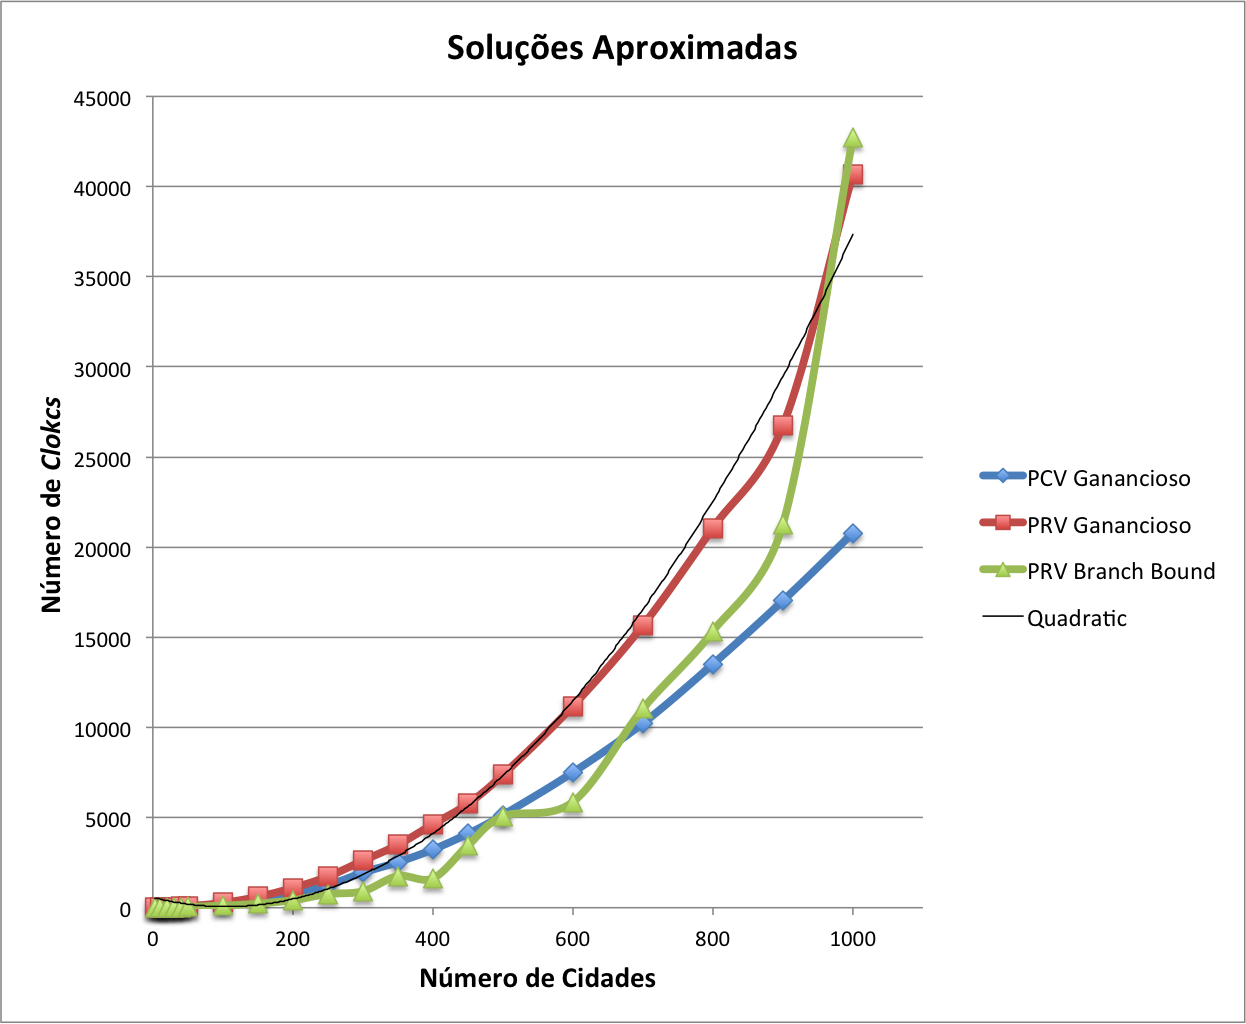
\includegraphics[width=15cm]{aprox.png}
\caption{Complexidade temporal dos algoritmos aproximados}
\label{aprox}
\end{center}
\end{figure}

Em relação aos algoritmos exatos, tal como esperado, a complexidade temporal observada é fatorial, como demonstra a Figura~\ref{exact}. Note-se que a escala do número de ciclos do relógio é logarítmica, por isso é que a função exponencial é representada por uma reta. Já as interpolações dos resultados obtidos, crescem bem mais do que a exponencial, como se pode observar melhor na Figura~\ref{exact2}, em que a escala é normal. Em relação ao desempenho relativo entre estes algoritmos, no PCV a optimização não ajuda, mas no PRV permite obter um desempenho consideravelmente melhor, apesar de a complexidade ser a mesma.

\begin{figure} [ht]
\begin{center}
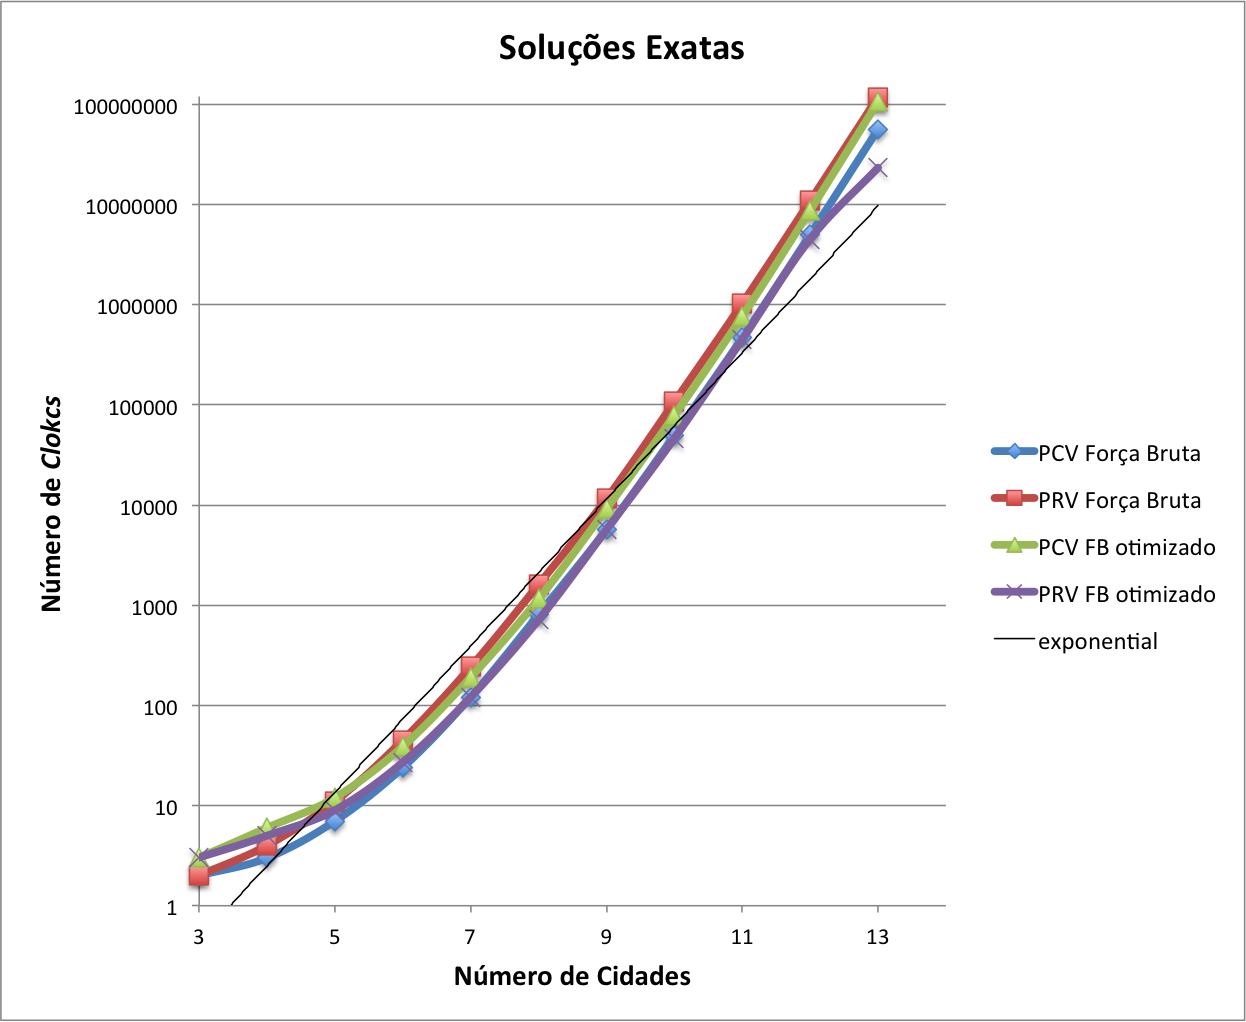
\includegraphics[width=15cm]{exact.png}
\caption{Complexidade temporal dos algoritmos exatos - escala logaritmica}
\label{exact}
\end{center}
\end{figure}

\begin{figure} [ht]
\begin{center}
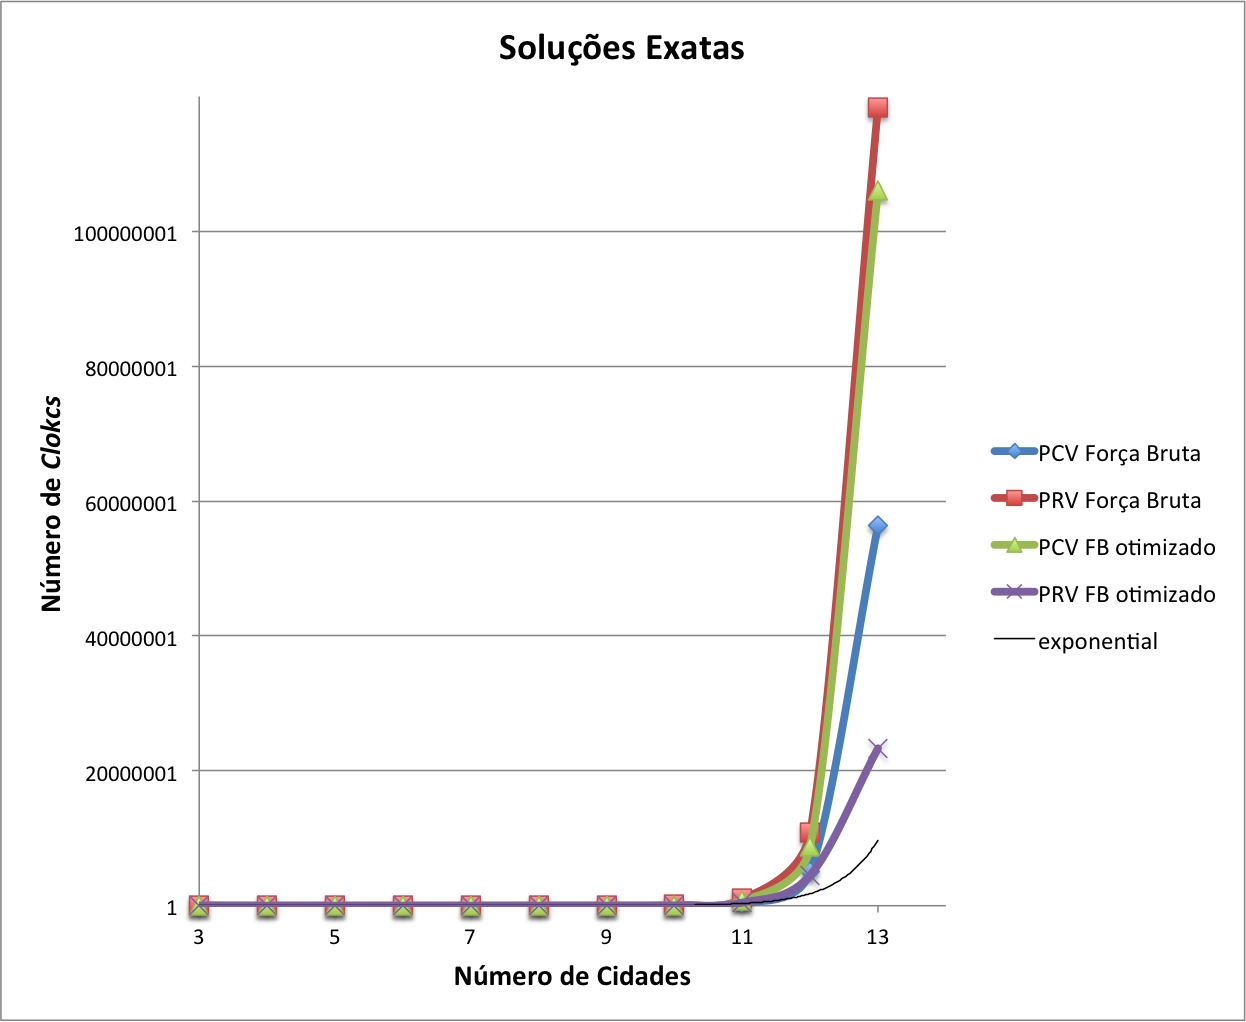
\includegraphics[width=15cm]{exact2.png}
\caption{Complexidade temporal dos algoritmos exatos - escala normal}
\label{exact2}
\end{center}
\end{figure}

Estas diferenças de desempenho tão abismais, apontam para uma maior utilização dos algoritmos aproximados. Repare-se que os algoritmos exatos, a partir de 13 cidades começaram a demorar demasiado tempo para que fossem feitos os testes de complexidade. No entanto, antes de utilizar soluções aproximadas, é necessário estimar a sua qualidade. O método é semelhante ao teste de complexidade: utilizamos vários conjuntos de dados aleatórios, com várias dimensões, e calculamos para cada amostra a diferença entre a solução exata e a solução aproximada.

Os resultados foram bastante interessantes. Em dados aleatórios em que os tempos de percurso possam variar bastante, o algoritmo ganancioso para o PCV encontra uma solução 32\% pior que a solução exata e o algoritmo \emph{branch and bound} é 42\% pior que o exato para o PRV. Mas se as distancias entre as cidade não variarem muito, o PRV tem uma solução aproximada 3\% pior e o PRV tem uma solução aproximada 27\% pior. Já a solução gananciosa para o PRV é apenas 3\% pior que a solução exata, independentemente das distâncias serem semelhantes ou não.

Estes dados levaram-nos a escolher como algoritmos principais para o PRV a solução exata se o número de cidades for no máximo 10 e a solução gananciosa a partir daí.

%%%%%%%%%%%%%%%%
% DIFICULDADES %
%%%%%%%%%%%%%%%%
\chapter{Principais Dificuldades}

A parte do problema com um tempo limite para fazer a viagem não parece ser muito conhecida. De facto, não chegamos a encontrar nenhum problema análogo ao nosso, mesmo a informação sobre o Problema de Roteamento de Veículos parece focar-se em problemas ligeiramente diferentes. Mais, este problema é pelo menos tão difícil como a versão sem tempo limite. De facto, se o tempo limite for suficientemente grande, passamos a calcular o melhor percurso para visitar todas as cidades, em vez de escolher um subconjunto de cidades a visitar. Por isso fomos obrigados a tratar os dois problemas em conjunto, o que complicou a tarefa.

Por outro lado, a formulação/escolha de algoritmos concretos e o modelo a utilizar são dependentes um do outro, o que gerou uma maior incerteza inicial sobre como abordar a resolução do problema. Logo à partida, a escolha do tipo de grafo a usar gerou algumas confusões. Havia várias hipóteses e cada uma delas necessitava de ser tratada de diferente forma, fazendo o uso de algoritmos diferentes. Ao ponderar possíveis resoluções, pequenas ideias que intuitivamente pareciam corretas eram frequentemente falaciosas. Além disso, tentar conciliar diferentes técnicas para chegar a um algoritmo relativamente eficiente parecia uma tarefa impossível.

Apesar deste atrito inicial, existe bastante informação disponível sobre problemas ligados a grafos e desde cedo tivemos conhecimento do Problema do Caixeiro Viajante, que nos levou a escolher um grafo completo e consequentemente simplificar a análise do problema. A ajuda dos docentes também se verificou valiosa na formulação de soluções.

%%%%%%%%%%%%%
% CONCLUSAO %
%%%%%%%%%%%%%
\chapter{Conclusão}

Esta fase inicial de pesquisa e formulação de soluções permitiu aprofundar o conhecimento relativo a problemas similares e possíveis resoluções. A equipa foi exposta a alguns dos algoritmos a ser implementados na próxima fase do trabalho prático e já tem uma noção geral de como prosseguir.

Ficamos também com maior sensibilidade face à escolha dos tipos de dados a usar, nomeadamente no que diz respeito às restrições consideradas e até que ponto ajudam a encontrar algoritmos mais eficientes.

Será certamente gratificante passar tudo isto à prática numa próxima fase do trabalho, embora a quantidade de algoritmos diferentes que estamos a considerar faça esta tarefa parecer hercúlea. Eventualmente será necessário optar por apenas alguns destes caminhos, consoante a dificuldade de implementação e a promessa de eficiência de cada um. n

%%%%%%%%%%%%%%%%
% BIBLIOGRAPHY %
%%%%%%%%%%%%%%%%
\bibliographystyle{IEEEtran}
\bibliography{rabb,refs}

\end{document}
